\section{Auswertung}
\label{sec:Auswertung}

\subsection{Detektorscan}
Zunächst wird der Detektorscan analysiert. 
Dafür werden die Messwerte in \autoref{fig:Detektorscan} aufgetragen.
Die Intensität gibt dabei die Anzahl der gemessenen Photonen pro Zeiteinheit an, in diesem Teil des Versuchs pro Sekunde.
\begin{figure}
    \centering
    \caption{Die aufgenommenen Intensitätsmesswerte werden gegen den Winkel aufgetragen. Zudem wird eine Gauß-Verteilung an die Werte angepasst und daraus die Halbwertsbreite und das Intensitätsmaxium berechnet und makiert.}
    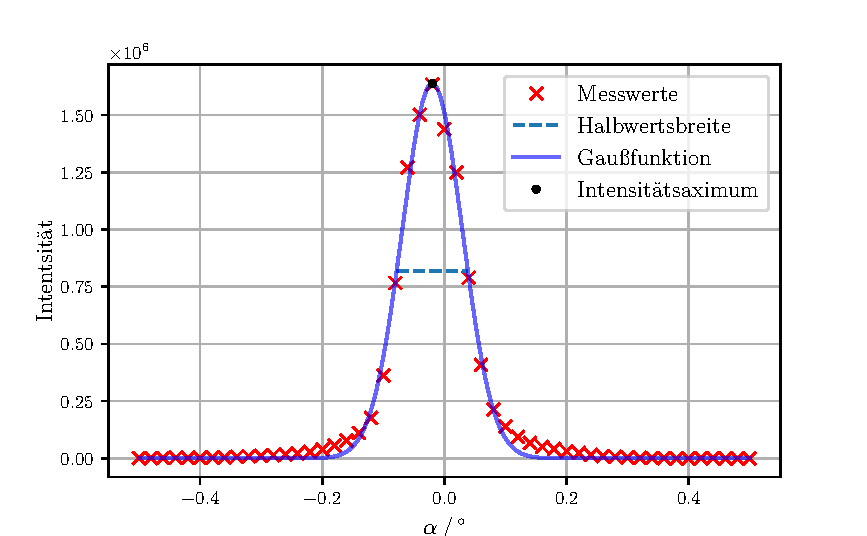
\includegraphics[width=\textwidth]{content/data/Detectorscan.pdf}
    \label{fig:Detektorscan}
\end{figure}
An die Messwerte wird eine Gauß-Verteilung angepasst.
Dazu wird das python Paket \cite{scipy} genutzt.
Dieses führt eine Ausgleichsrechung für die Funktion 
\begin{equation*}
    I(\alpha) = \frac{a}{\sqrt{2\pi\sigma^2}} \exp{\frac{-\left (\alpha- \mu \right)^2}{2\sigma^2}}
\end{equation*}
mit den Messwerten durch.
Die Ausgleichsrechung hat die Werte 
\begin{align*}
    a =& 1637959.863\\
    \sigma =& 20.205 \\
    \mu =& -0.019 \\
\end{align*}
ergeben.
Die dadurch definierte Gauß-Verteilung ist ebenfalls in \autoref{fig:Detektorscan} zu sehen.
Aus dieser wird das Intensitätsmaxium $I_\text{max}$ und die Halbwertsbreite $FWHM$ bestimmt.
Die bestimmten Werte sind
\begin{align*}
    I_\text{max} =& \SI{1637959.685}{\per \second} \\
    FWHM =& \SI{0.116}{\degree}.\\
\end{align*}
\FloatBarrier
\subsection{Z-Scan}
Die Messwerte des Z-Scans sind in \autoref{fig:zscan} zu sehen.
Da nicht alle Werte für die Auswertung relevant sind werden nur die Werte zwischen $z = -0.4 \text{\, bis \, } 0.7 \, \si{\milli\meter}$ geplottet.
\begin{figure}
    \centering
    \caption{Die relevanten Messwerte des Z-Scans. Zudem wurden durch gründe Linien die Strahlbreite makiert.}
    \includegraphics[width=\textwidth]{content/data/zscan.pdf}
    \label{fig:zscan}
\end{figure}
In der \autoref{fig:zscan} ist zudem die Strahlbreite $d_0$ in grün makiert.
Der Strahl hat eine Breite von 
\begin{align*}
    d_0 =& \SI{0.24}{\milli\meter}.
\end{align*}

\subsection{Rockingscan}
Die Messwerte der Rockingscans sind in \autoref{fig:rockingscan} zu finden.
\begin{figure}
    \centering
    \caption{Die Messwerte des Rockingscans und die makierten Geometriewinkel.}
    \includegraphics[width=\textwidth]
    \label{fig:rockingscan}
\end{figure}
In grün sind in der \autoref{fig:rockingscan} die Geometriewinkel $\alpha_\text{g}$ makiert.
Zudem wird aus dem Geometriewinkel links und rechts ein Mittel $\bar{\alpha_\text{g}}$ gebildet.
Die Geometriewinkel haben einen Wert von 
\begin{align*}
    \alpha_\text{g, links} =& \SI{-0.560}{\degree}
    \alpha_\text{g, rechts} =& \SI{0.560}{\degree}
    \bar{\alpha_\text{g}} =& \SI{0.560}{\degreeS}.
\end{align*}
Aus der Strahlbreite und der Länge der Probe $D=\SI{20}{\milli\meter}$ ist es zudem möglich den theoretischen Geometriewinkel zu berechnen.
Dies geschieht mit Gleichung \eqref{eq:Geometriewinkel}.
Der daraus resultierende theoretische Geometriewinkel beträgt
\begin{align*}
    \alpha_\text{g, theo} =& \SI{0.687}{\degree}.
\end{align*}

\subsection{Reflektivitätsmessung}
